% ICASSP 2027 manuscript. Quantitative tables/figures are auto-generated from
% frozen result CSVs by scripts/make_paper_assets.py into assets/; every
% numerical claim is traceable to assets/paper_claims.json and source CSVs.
\documentclass{article}
\usepackage{spconf,amsmath,amssymb,graphicx,hyperref}
\usepackage{xcolor}
\def\x{{\mathbf x}}
\def\L{{\cal L}}

% ---- include an auto-generated table only if it exists ----
\newcommand{\inputtable}[1]{\IfFileExists{assets/tables/#1}{\input{assets/tables/#1}}{\emph{(table pending: \detokenize{#1})}}}
\setlength{\intextsep}{6pt plus 2pt minus 2pt}
\setlength{\abovecaptionskip}{4pt}
\setlength{\belowcaptionskip}{1pt}

\title{AUDITING STRUCTURED POLICY LEARNING FOR STREAMING TRANSACTION
COLLATERAL CONTROL: FACTORIZATION, CONDITIONING, AND CROSS-SCALE TRANSFER}

\name{\begin{tabular}{@{}c@{}}Sijia Zhou$^{1,\dagger}$, Yingda Yu$^{1,\dagger}$, Jiaqi Xuan$^{1}$, Zhentong Ye$^{2}$, \\ Jia Rong$^{1}$, Caiming Zhao$^{1}$, Siaxia Chen$^{3}$, Guanchao Tong$^{1,*}$\end{tabular}}
\address{$^{1}$Wenzhou-Kean University, Wenzhou, China \\
$^{2}$Northwestern University, Evanston, IL, USA \\
$^{3}$Adelphi University, Garden City, NY, USA \\
$^{\dagger}$Equal contribution \\
$^{*}$Corresponding author}

\begin{document}
\ninept
\maketitle

\begin{abstract}
Off-chain payment nodes route a stream of transactions into $k$
collateralized wallets and periodically pay to flush a wallet. We treat the
resulting collateral-control task as an online sequential decision problem over
nonstationary transaction streams and audit, in a controlled multi-seed
reimplementation, which structural inductive biases help a learned PPO
controller. Three questions organize the study: whether factoring the joint
(settle, flush) action into two heads improves on a quadratic joint head;
whether conditioning the flush head on the planned settle action adds value;
and whether a permutation-equivariant, $k$-independent encoder enables
deployment across wallet counts. Across five seeds and four collateral
budgets, factorization is the reliable effect: the settle-conditioned
factored policy beats the joint head at every budget and the independent
variant at most budgets, whereas zero- and shuffled-conditioning ablations
detect no benefit from the settle-to-flush path. The equivariant encoder
loads and runs zero-shot at unseen wallet counts, although transfer
quality is asymmetric. A single validation-selected
balance-feedback rule remains the strongest tested controller, both on
stationary streams and across abrupt regime switches.
\end{abstract}

\begin{keywords}
reinforcement learning, structured policies, streaming resource allocation,
online sequential decision making, payment-channel networks, nonstationary
transaction streams, permutation equivariance.
\end{keywords}

\section{Introduction}
Off-chain payment networks such as the Lightning
Network~\cite{poon2016lightning,miller2019sprites,kolachala2024sok} process
streams of transactions over wallets backed by finite collateral, and routing
under scarce channel funds has been studied for payment channel
networks~\cite{sivaraman2020spider}; reinforcement learning has more recently
been applied to PCN scheduling, paid rebalancing and hybrid
pathfinding, and liquidity
placement~\cite{papadis2023rebalancing,chen2024drlpcr,mishra2025relearn,valko2025hybrid}.
Transactions arrive sequentially, each
with a requested value, and at every arrival the node must either settle it
into one of $k$ wallets that currently holds enough free balance or drop it;
independently, it may \emph{flush} one wallet, paying a fixed fee to empty and
recharge it while the wallet briefly cannot accept funds. The problem is
inherently sequential: a flush frees capacity for future arrivals but costs
money and removes a wallet from service, while greedily accepting now can
starve a later, larger transaction. The task thus combines streaming
observations, structured discrete actions, and online resource allocation
under nonstationary transaction arrivals. Collateral is partitioned per wallet
rather than pooled, and future arrivals are unknown. Such sequential
decisions are the domain of online competitive
analysis~\cite{borodin1998online} and its learning-augmented
variants~\cite{lykouris2018competitive}; the closest formal model, online
collateral maintenance with $k$ wallets of capacity $C/k$, admits worst-case
competitive guarantees~\cite{almashaqbeh2024competitive}, alongside PCN
topology-and-admission analyses~\cite{chatterjee2025boosting} and related
online-inventory results~\cite{lin2019competitive}.

This structure makes a naive policy parameterization costly. A joint
categorical controller emits one logit per (settle, flush) pair,
$(k{+}1)^2$ outputs at $k{=}24$, allocating capacity to pairs that are
conflicting or dominated even though the two decisions are only weakly
coupled. Branched and factorized action heads address precisely this
issue~\cite{tavakoli2018action}. Factorization is therefore the natural
structural move: two smaller $k{+}1$-way heads reduce the output count to
$2(k{+}1)$. A residual question is whether the coupling between the two
choices matters---specifically, whether conditioning the flush decision on the
\emph{planned} settle wallet (a directed settle$\to$flush information path)
adds value. We treat this mechanism as a hypothesis to test rather than a
feature to assume.

A second structural question arises at deployment. The wallet count $k$ is an
operating condition that can change between deployments, yet a flat multilayer
perceptron bakes $k$ into its weight shapes: a model trained at one $k$ cannot
be loaded at another. Encoding the wallets as an unordered set with a shared,
permutation-equivariant function removes all $k$-dependent parameters and
allows one trained policy to be deployed zero-shot at a new wallet count.
Whether such portability carries a matched-scale accuracy cost is, again, an
empirical question.

The ingredients are established, but their payoff here is not. Factored and
large discrete action policies remove combinatorial output growth through
factorized distributions and Q-decompositions~\cite{tang2020discretizing,lee2025factored}
or stochastic subset search~\cite{fourati2024stochastic}; permutation-invariant
set processing is supplied by sum-based and attention-based set
encoders~\cite{zaheer2017deepsets,lee2019settransformer}; and RL has been used
for PCN routing, relay-node rebalancing, and liquidity
allocation~\cite{sivaraman2020spider,papadis2023rebalancing,chen2024drlpcr,mishra2025relearn}.
Building on these established primitives, we conduct a controlled empirical
audit of which structural biases improve streaming collateral control:
matched mechanism ablations, zero-shot cross-$k$ deployment, a strong
validation-selected feedback baseline, and paired multi-seed evaluation, with
null results reported alongside positive ones.

Finally, learned controllers should be assessed against a baseline that uses
the most informative available signal, namely current wallet fill. We
therefore include a validation-selected balance-feedback rule on equal
footing with the learned policies. All questions are answered on a faithful
port of the original K-Wallet environment and its twelve-regime traffic
generator with matched seeds and paired confidence intervals; null results
are reported together with positive ones.

\noindent Our contributions are:
\begin{itemize}
\item A controlled five-seed audit of joint versus factorized PPO action
parameterizations (joint head, independent heads, settle-conditioned heads),
including matched zero/shuffle mechanism ablations, on a faithful, tested
port of the environment and the twelve-regime generator.
\item A permutation-equivariant set encoder with no $k$-dependent parameter
(in the spirit of Deep Sets~\cite{zaheer2017deepsets}), which loads and runs
zero-shot at unseen wallet counts where a fixed-shape flat MLP cannot reuse
its weights, together with an explicit account of its transfer asymmetry.
\item A comparison against a validation-selected balance-feedback baseline on
both stationary streams and abrupt regime switches, including per-seed paired
tests and Holm-corrected significance statements.
\end{itemize}

\section{Streaming collateral control}
Collateral $C\in\{800,900,1000,1200\}$ is split into $k{=}24$ homogeneous
wallets of capacity $C/k$; transfer experiments additionally use
$k\in\{6,12\}$. At each of $T{=}1000$ decisions a transaction of size
$x_t\in[0,1000]$ arrives. Wallet $i$ is described by
$z_{i,t}=(\text{balance}_i,\text{availability}_i,\text{cooldown}_i)$, and two
global scalars $g_t=(\tilde x_t,t/T)$ give the normalized transaction size and
time progress; the observation is the concatenation, of dimension $3k{+}2$.
The controller chooses $a_s,a_f\in\{1,\ldots,k\}\cup\{\bot\}$, a settle
wallet and a flush wallet (null $=$ no-op). A flush executes \emph{first}: the
selected wallet is charged, made unavailable for $F{=}3$ decisions, and then
refilled to full; the transaction is settled afterwards, accepted if $a_s$ is
usable and holds free balance at least $x_t$, and dropped otherwise. Flushing
and settling the same wallet is not forbidden, but the flushed wallet is in
cooldown when settlement is attempted, so such conflicting pairs typically
drop the transaction. Drops are attributed as \emph{oversize} ($x_t>C/k$,
infeasible for any policy), \emph{frozen} (settle wallet in cooldown), or
\emph{avoidable} (insufficient balance or a flush/settle conflict that
proactive flushing could have prevented). Per-episode Money is
\begin{equation}
M \;=\; p\sum_t x_t\,\mathbb{1}[\text{accepted at }t]
   \;-\; \tau\sum_t \mathbb{1}[a_{f,t}\neq\bot],
\end{equation}
with acceptance price $p{=}1$ and flush fee $\tau{=}10$; a drop carries no
additional penalty. A stochastic policy is optimized with episodic
PPO~\cite{schulman2017ppo} and generalized advantage
estimation~\cite{schulman2015gae}, and evaluated deterministically (argmax)
on fixed episode pools. Episodes are generated with fixed seeds from twelve
regimes spanning steady, large-transaction, and correlated-burst traffic:
$5000$ training, $300$ validation, and $200$ test episodes per regime. Every
method and seed uses the same deterministic test pools; the statistical unit
is the matched training seed ($n{=}5$ main, $n{=}3$ ablations/switching), not
the individual test episodes. All design choices use validation only, and
failed seeds are retained (Fig.~\ref{fig:overview}).

\begin{figure}[t]
\centering
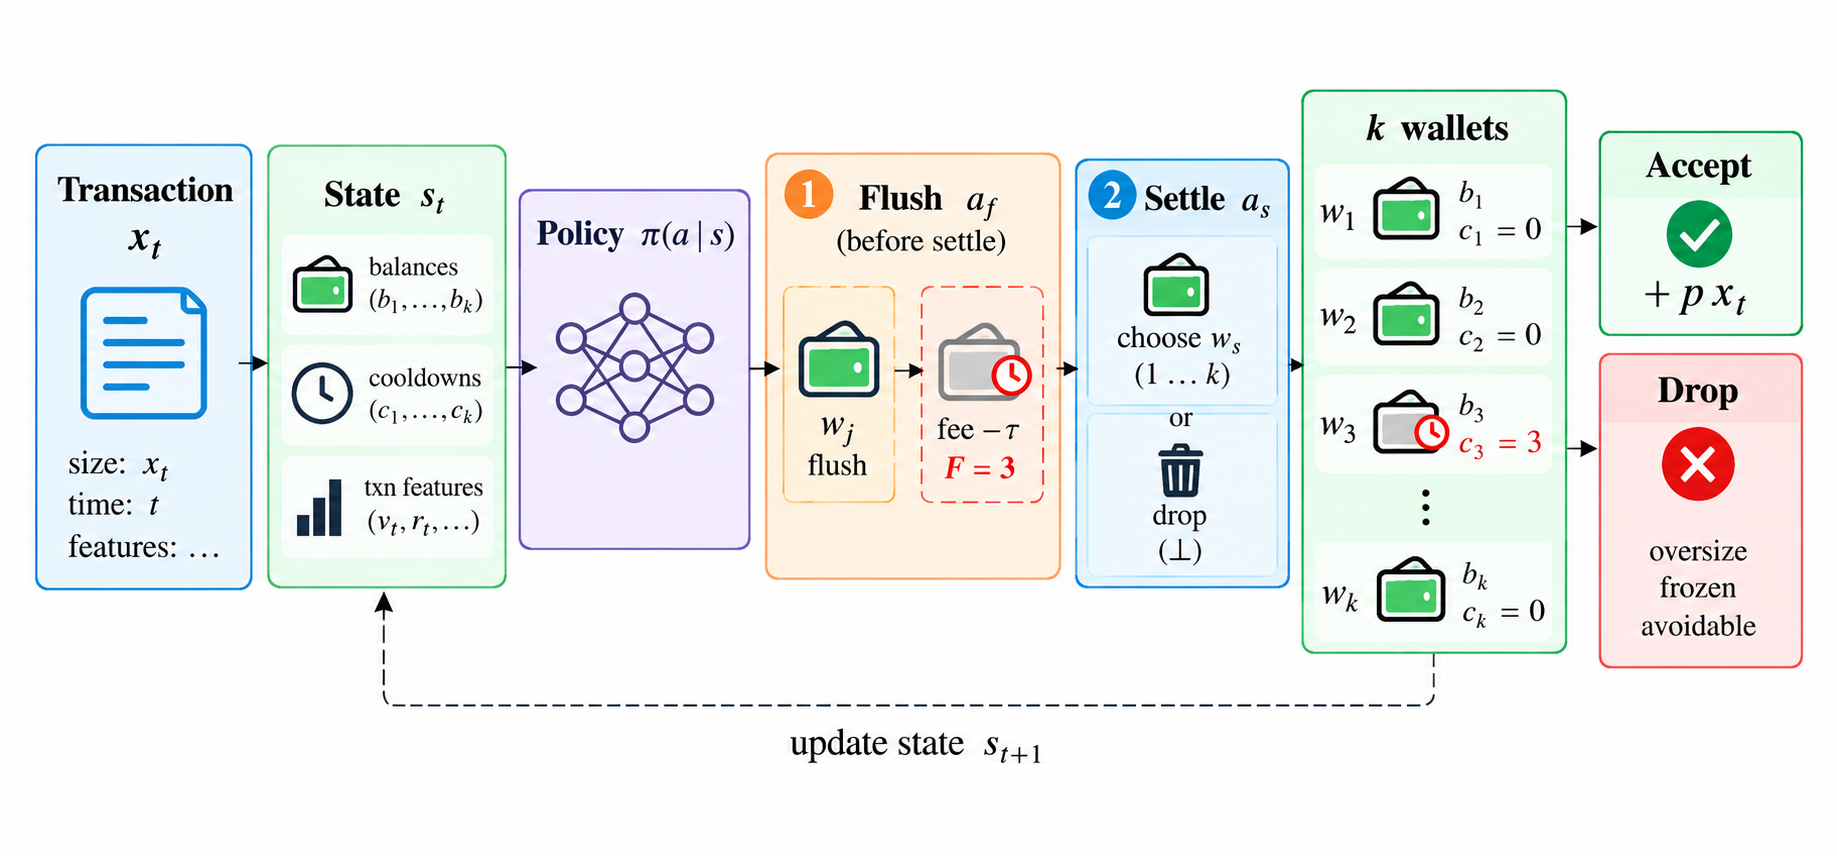
\includegraphics[width=0.98\columnwidth]{assets/figs/fig1_chatgpt.png}
\caption{One collateral-control decision. The policy selects a settle action
and a flush action; the environment executes the flush first (fee $\tau$,
cooldown $F$) and settlement second. Accepted value earns $p x_t$; drops are
oversize, frozen, or avoidable (the binary availability indicator is not
drawn in $s_t$).}
\label{fig:overview}
\end{figure}

\section{Policies}
\noindent\textbf{JA-PPO} emits one categorical over all settle/flush pairs,
$(k{+}1)^2$ logits ($625$ at $k{=}24$). It treats the step as one large joint
decision, which inflates the output layer and assigns probability mass to
conflicting or dominated pairs. Structured large-action spaces have been
addressed with action embeddings~\cite{dulac2015deep}, parameterized-action
hierarchies~\cite{hausknecht2016deep}, action
branching~\cite{tavakoli2018action}, factorized on-policy distributions and
Q-decompositions~\cite{tang2020discretizing,lee2025factored}, stochastic
subset maximization~\cite{fourati2024stochastic}, and neighborhood
construction~\cite{akkerman2024dynamic}.

\noindent\textbf{IFAC} factors the action into two independent $k{+}1$
categoricals, $\pi(a_s,a_f\mid s)=\pi_s(a_s\mid s)\,\pi_f(a_f\mid s)$ (50
logits), sharing a trunk. This removes the quadratic head, encodes the
weak-coupling prior between the sub-decisions, and lets each head learn from
its own signal at every step instead of from rarely observed joint pairs.

\noindent\textbf{SC-FAC} keeps the factorization and adds a directed
settle$\to$flush path. At the \emph{policy level} a settle action $a_s$ is
first sampled (or selected, under deterministic evaluation); an embedding
$e(a_s)$ of that planned action then conditions the flush distribution,
$\pi_f(a_f\mid s,a_s)$. The intended mechanism is coordination---in
particular, avoiding a flush of the wallet selected for the imminent
settlement and choosing complementary flush/settle pairs. This conditioning
is a dependency within the policy, not an execution order: the environment
still executes $a_f$ before $a_s$, and no value has been moved when $a_f$ is
chosen. Two matched ablations share the architecture exactly:
\textbf{no-cond.} zeroes $e(a_s)$ and \textbf{shuffled} supplies a deranged
(wrong-wallet) embedding.

\noindent\textbf{Set encoder.} The wallets are intrinsically an unordered
set. A shared function first encodes each wallet jointly with the global
context, $h_i=\phi(z_i,g_t)$; symmetric pooling gives
$\bar h=\rho(\{h_j\}_{j=1}^{k})$ (mean pooling). Per-wallet settle and flush
logits are then
\[
\ell_i^{s}=\psi_s(h_i,\bar h,g_t),\qquad
\ell_i^{f}=\psi_f(h_i,\bar h,g_t,e(a_s)),
\]
while the no-op logits are produced from global context $(\bar h,g_t)$ alone
(for SC-FAC, $e(a_s)$ is the gathered feature $h_{a_s}$, zero for
$a_s=\bot$). Because $\phi,\rho,\psi_s,\psi_f$ are shared across wallets and
no tensor is sized by $k$, the map is permutation-equivariant and its weights
can be loaded and executed at any wallet count without retraining---the
property a flat MLP lacks; attention-based set
encoders~\cite{lee2019settransformer} offer the same invariance with pairwise
interactions (Fig.~\ref{fig:structures}).

\begin{figure*}[t]
\centering
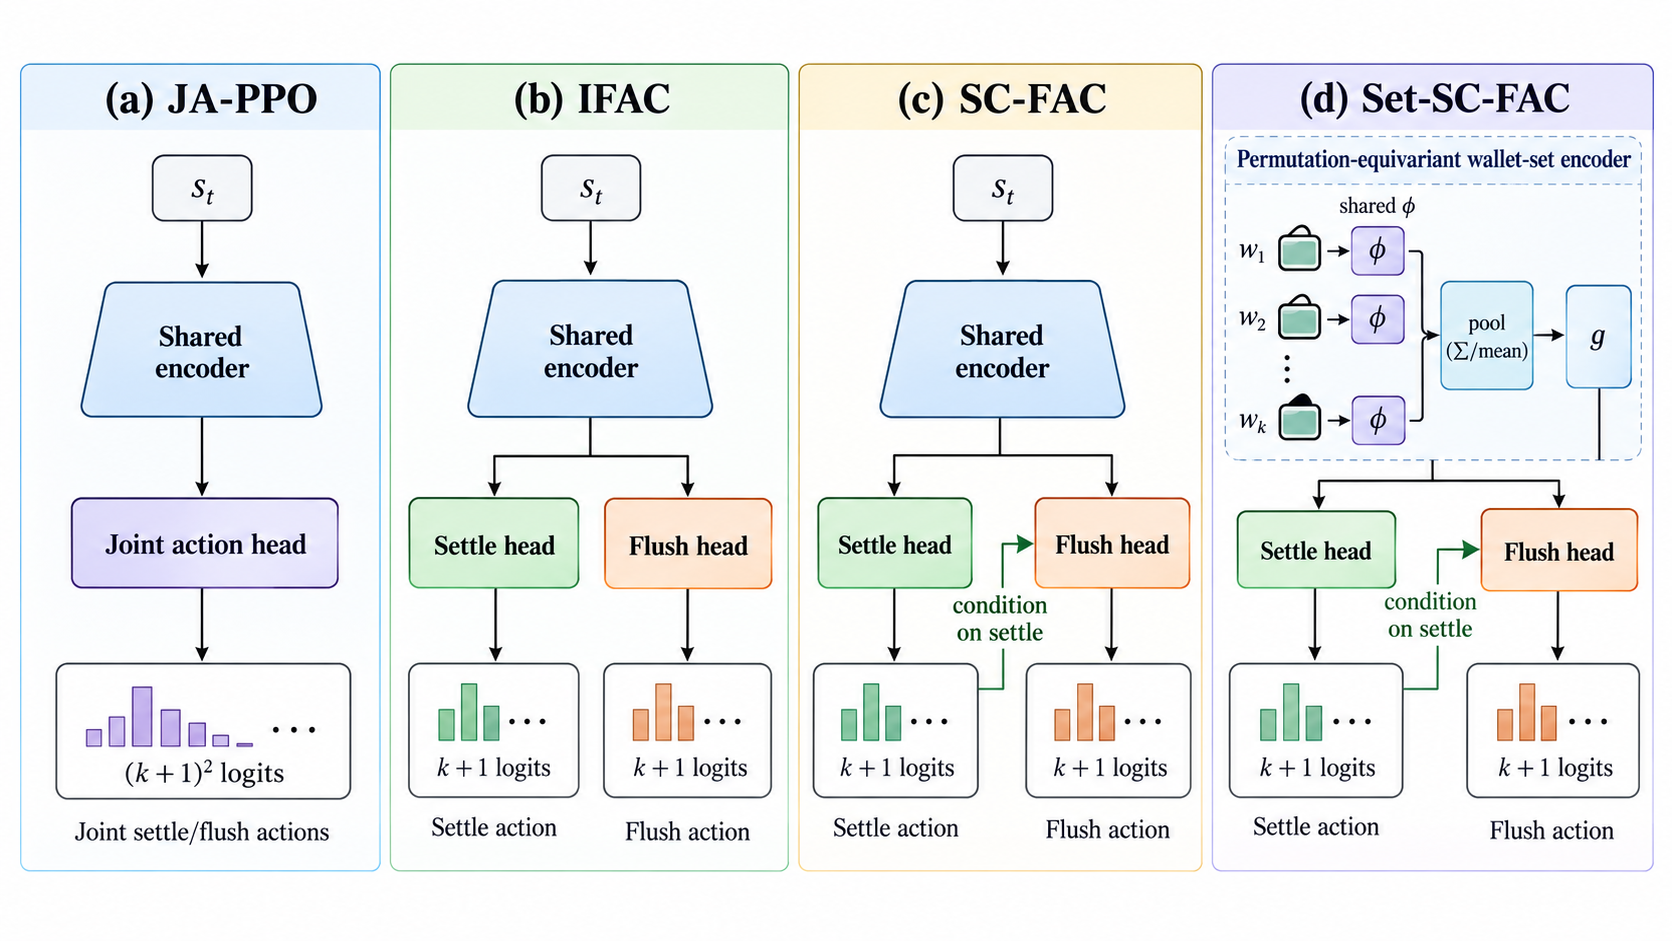
\includegraphics[width=0.92\textwidth,trim=0.55cm 2.30cm 0.50cm 2.05cm,clip]{assets/figs/fig2.png}
\caption{Action parameterizations: (a) JA-PPO, one joint head over
$(k{+}1)^2$ outcomes; (b) IFAC, independent settle/flush heads; (c) SC-FAC,
flush conditioned on the sampled $a_s$; (d) Set-SC-FAC, shared per-wallet
encoder with symmetric pooling. Conditioning is a policy-level dependency;
execution stays flush-before-settle.}
\label{fig:structures}
\end{figure*}

\section{Experiments and results}
All policies are evaluated deterministically on fixed, shared test pools;
model and training choices use validation only. Inference uses paired $t$
tests on matched seeds, and we additionally report Holm step-down adjusted
$p$-values within pre-specified contrast families; these corrections are
exploratory, as the study was not powered for them. Rule baselines are the
native one-flush references FA and FWF (reconstructed, since the reference
design allowed multiple flushes per step), a rotation rule (ROT), and the
balance-feedback policy \textbf{BFP}. It settles into the usable (non-cooling)
wallet with the smallest remaining free balance that covers $x_t$ (best
fit), and in the same step flushes the most depleted usable wallet other
than the settle wallet when its free balance satisfies $b_i<\theta C/k$; if
nothing fits, it flushes the most depleted usable wallet and the transaction
drops. A single threshold $\theta{=}0.5$ was selected once, by mean Money
over $\theta\in\{0.3,0.5,0.8\}$, on the $300$-episode mixed validation pool
($25$ episodes per regime), then frozen and used unchanged at all four
capacities; test pools were never used for tuning. We also report an oracle
feasible value and the drop decomposition.
\noindent\textbf{Implementation details.} All learned policies share one PPO
configuration: a two-layer trunk with $256$ hidden units (a $32$-dimensional
settle embedding in SC-FAC), Adam at $3{\times}10^{-4}$, discount
$\gamma{=}0.99$, GAE $\lambda{=}0.95$, clipping $\epsilon{=}0.2$, value
coefficient $0.5$, entropy coefficient linearly annealed
$0.02{\to}0.001$, and gradient-norm clipping at $1.0$. Each run trains for
$3000$ episodes collected in $8$-episode rollouts, with $10$ update epochs
and $512$-transition minibatches. Checkpoints are selected by deterministic
Money on validation, and every reported number uses deterministic
($\arg\max$) evaluation on the shared test pools. Main seeds are
$123,323,532,777,999$; ablation and switching runs use the first three.

\noindent\textbf{Factorization and the strong baseline.}
Table~\ref{tab:main} reports Money per capacity; the seed-level paired
contrasts at $C{=}1200$ are stated in this paragraph. Every method incurs the same
structural oversize floor of about $400$ drops per episode; the policy
differences lie in the avoidable fraction, which at $C{=}1200$ falls from
$77.0$ drops/episode for JA-PPO to $49.5$ (IFAC) and $40.4$ (SC-FAC).
\emph{Factorization is the reliable learned effect.} SC-FAC outperforms
JA-PPO at all four capacities ($+677$, $+999$, $+1327$, $+1285$ Money;
$p=0.012,0.0067,{<}0.001,0.004$; $5/5$ seeds), and all four contrasts survive
Holm correction (adjusted $p=0.036,0.027,0.0003,0.022$). IFAC outperforms
JA-PPO at $C\in\{800,900,1200\}$ in raw tests ($p<0.001,0.032,<0.001$) but not
at $C{=}1000$ ($p=0.57$); after Holm correction only $C\in\{800,1200\}$
remain significant ($C{=}900$ adjusted $p=0.064$). The added settle-conditioning
path does not account for this gain: the SC-FAC$-$IFAC contrast includes zero
at $C\in\{900,1000,1200\}$, and at $C{=}800$ SC-FAC is lower ($-419$,
$p=0.009$). The parameterization itself is smaller as well as stronger:
outputs drop from $625$ to $50$ logits and the actor from $245{,}874$ to
$98{,}099$ parameters (IFAC); the set variants use about $135$k parameters
with no $k$-dependent tensor and sub-millisecond per-step CPU latency.
\emph{The feedback rule sets the level to beat.} BFP attains the highest
Money at every capacity with zero avoidable drops, and its advantage is
significant in $11$ of $12$ method-capacity paired contrasts after Holm
correction; the sole exception is versus IFAC at $C{=}1000$ ($+2545$,
$p=0.057$, 95\% CI including zero), which BFP nevertheless wins on all five
seeds.

\begin{table}[htb]
\centering
\footnotesize
\setlength{\tabcolsep}{3.6pt}
\inputtable{main_results.tex}
\caption{Money per episode (mean$\pm$SE over $n{=}5$ training seeds) versus
collateral $C$. Rules need no seeds.}
\label{tab:main}
\end{table}

\noindent\textbf{Settle-conditioning mechanism.}
Table~\ref{tab:abl} compares SC-FAC with the no-conditioning and
shuffled-conditioning variants under matched parameters, seeds, and budget at
$C{=}1200$; the corresponding paired intervals all include zero
($-284$ with CI $[-1678,1110]$, $p=0.47$; $-301$ with CI $[-1212,611]$,
$p=0.29$), as do the matched contrasts at $C{=}800$ (raw $p=0.27$ and $0.65$); all
Holm-adjusted values are $1.0$. The fully conditioned variant also spends
marginally more on flushes without higher accepted value. At the tested flush
price and observation model, the identity of the planned settle wallet carries
no detectable additional decision-relevant signal once wallet state is
observed.

\begin{table}[htb]
\centering
\footnotesize
\inputtable{ablation.tex}
\caption{Settle-conditioning mechanism ablations ($C{=}1200$; same $n{=}3$
seeds per variant).}
\label{tab:abl}
\end{table}

\noindent\textbf{Cross-$k$ transfer and regime shifts.}
We train at $k\in\{6,12,24\}$ and deploy, with no retraining, at every $k$.
Table~\ref{tab:xfer} shows that the set encoder loads and runs at every
deployment $k$, including all six zero-shot off-diagonal cells (Money from
$4433$, $k{=}6{\to}24$, to $43733$, $k{=}12{\to}6$), where a flat policy has
no entry because its weight shapes change with $k$. The benefit is operational
deployability rather than uniformly preserved performance: zero-shot
retention is asymmetric, strongest toward larger-wallet operating points and
weakest when a model trained with large wallets meets the small wallets at
$k{=}24$ (e.g.\ $k{=}6{\to}24$ yields $4433$). At matched $k$ the set encoder
is slightly above the flat MLP at $k{=}6$ ($46742$ vs.\ $44820$) and $k{=}12$
($36391$ vs.\ $34193$). At $k{=}24$ the primary all-seed Set-SC-FAC mean is
$9190$ versus $13610$ for the flat model, and includes one failed Set-SC-FAC
run (seed $532$, Money $0$), retained in the primary aggregate; a
sensitivity calculation over the two nonfailed set runs yields $13785$
(flat MLP $n{=}3$), which we report only as a sensitivity analysis.

\begin{table}[t]
\centering
\footnotesize
\setlength{\tabcolsep}{3.8pt}
\inputtable{transfer_compact.tex}
\caption{Cross-$k$ Money (Set-SC-FAC): rows train $k$, columns deploy $k$;
$^{\dagger}$zero-shot deployment. Diagonal cells also show the matched flat
MLP in parentheses; the flat MLP fills only those three diagonal cells because
its tensors are $k$-shaped.}
\label{tab:xfer}
\end{table}

For regime shifts, every policy is trained on stationary pools only and
tested on identical deterministic episodes spliced across regimes at an
abrupt change point (six scenarios~\cite{gama2014survey}:
calm$\leftrightarrow$burst, early and late). Table~\ref{tab:sw} reports
post-switch avoidable drops and Money. BFP incurs zero avoidable drops after
every switch and the highest Money, retaining its behavior without retraining.
The learned policies transfer substantially better than the naive rule
references ($28$--$56$ versus $144$--$148$ post-switch drops). Against BFP,
JA-PPO and IFAC remain worse on both metrics over the six paired scenarios
(one-sample paired tests, $n{=}3$; Holm-adjusted $p\le0.026$); for SC-FAC the
drops contrast is not significant ($p=0.088$), and its raw Money contrast
($p=0.035$) does not survive Holm correction ($p=0.069$). We therefore observe
robustness of the learned policies to the stream change, but no
switch-adaptation advantage over the tuned feedback rule.

\begin{table}[htb]
\centering
\footnotesize
\setlength{\tabcolsep}{4pt}
\inputtable{switching.tex}
\caption{Switching streams (mean over six scenarios; learned policies over
three seeds): total Money, post-switch Money, and post-switch recoverable
drops.}
\label{tab:sw}
\end{table}

\section{Discussion and conclusion}
Factoring the joint action into separate settle and flush heads is the
reproducible structural improvement in this study: gains over the quadratic
joint head survive multi-seed paired tests at every capacity for SC-FAC and at
two of four capacities for IFAC after Holm correction, coincide with a direct
reduction in avoidable drops, and reduce outputs from $(k{+}1)^2$ to
$2(k{+}1)$ and the actor to roughly $40\%$ of its parameters. In contrast,
the settle$\to$flush conditioning path shows no detectable Money benefit under
zero, shuffled, and matched-seed comparisons at the tested flush price.

The permutation-equivariant encoder provides a different property: operational
cross-$k$ deployability, allowing one trained policy to be loaded at wallet
counts the training never saw. Zero-shot retention is asymmetric. At
$k{=}24$, the all-seed result is strongly affected by one failed training
run, which is retained in the primary aggregate; this indicates training
instability and prevents a claim of matched-scale superiority. A practitioner fixed
at one wallet count gains little from the set parameterization; one who must
redeploy across changing counts gains portability that a fixed-shape network
cannot provide.

The validation-selected feedback rule is the strongest controller tested, on
stationary streams and after abrupt switches. On this homogeneous,
full-observation, i.i.d.-to-bursty workload, observable wallet fill therefore
captures much of the decision-relevant information. This bounds the setting
in which the learned policies have demonstrated an advantage; settings in
which richer temporal prediction is genuinely necessary---predictable
non-i.i.d. burst structure, heterogeneous wallet sizes or fees, multi-step
lookahead under expensive flushes---are the natural direction for future work.
Limitations are one flush per step, a finite horizon, one fixed fee, no
lookahead, homogeneous wallets, single-process PPO without vectorized
rollouts, and training instability at some $k$ (the retained failed seed).
The environment is a faithful port of the original (anonymous, unpublished)
K-Wallet specification, and policies together with unspecified
hyperparameters are documented re-implementations selected on validation;
the original manuscript's learned numbers are treated as reported rather
than regenerated.

\section*{Acknowledgment}
AI Usage Disclosure Statement. Generative AI tools were used solely to assist with
language polishing, grammatical correction, and improvements to the clarity and readability
of the manuscript. All research ideas, methodological design, implementations, experiments,
data collection and analysis, interpretation of results, figures and tables,
 and scientific conclusions were independently conducted, verified, and approved by the authors. 
 The authors take full responsibility for the accuracy, integrity, and content of the manuscript.

\clearpage
\bibliographystyle{IEEEbib}
\bibliography{refs}
\end{document}
